\documentclass[11pt,a4paper]{article}

\usepackage[T1]{fontenc}
\usepackage[utf8]{inputenc}
\usepackage[frenchb]{babel}

\usepackage{fancyhdr} % headers
\usepackage[usenames,dvipsnames]{color} % colors
\usepackage{graphicx} % images
\usepackage{listings} % source code
\usepackage{titling} % meta-infos
\usepackage{courier} % courier font
\usepackage{fullpage} % full page layout
\usepackage{titlesec} % title customization
\usepackage{parskip} % paragraphs spacing
\usepackage{amsmath}
\usepackage{tikz}
\usepackage{siunitx}
%\usepackage{showframe} % layout debug

\usepackage{float}
\restylefloat{figure}

\topmargin -10mm
\headsep 5mm
\headheight 10mm

\linespread{1.1}
\renewcommand{\arraystretch}{1.3}

%\setlength\parindent{0pt}
\setlength{\unitlength}{1cm}
\setlength{\droptitle}{-1.6cm}

\pagestyle{fancy}
\fancyhf{}
\cfoot{\thepage}

\def \doccourse { TIB1-B }
\def \doctitle {Rapport : NAT}
\author{Bastien Clément \and Christophe Peretti}

\renewcommand{\thesection}{Objectif \arabic{section} :}
\renewcommand{\thesubsection}{\arabic{section}.\arabic{subsection}}

\rhead{\theauthor \\ \today}
\lhead{\doccourse \\ \doctitle }
\title{{\normalsize \doccourse} \\ \doctitle }

\begin{document}

\maketitle
\vspace{1em}

\section{Configuration du réseau}

L'objectif de cette partie est de configurer les adresse IP des PCs et du routeur dans le simulateur. Il est atteint si nous pouvons envoyer des pings entre les différents PCs.

\subsection{Configuration du routeur Cisco}
\begin{tabular}{|r|l|}
	\hline	
	\textbf{Commande} & \textbf{Explication}  \\
	\hline
	\texttt{enable} & Passage en mode privilégié\\
	\texttt{configure terminal} & Passage en mode configuration globale\\
	\hline
	\texttt{interface FastEthernet0/0} & Accès à la configuration de l'interface interne\\
	\texttt{ip address 10.0.0.1 255.0.0.0} & Configuration de l'adresse ip de cette interface\\
	\texttt{no shutdown} & Activation de l'interface \\
	\texttt{exit} & Retour à la configuration globale \\
	\hline
	\texttt{interface FastEthernet0/1} & Accès à la configuration de l'interface externe \\
	\texttt{ip address 123.0.0.1 255.0.0.0} & Configuration de l'adresse ip de cette interface \\
	\texttt{no shutdown} & Activation de l'interface \\
	\texttt{exit} & Retour à la configuration globale \\
	\hline
	\texttt{exit} & Sortie du mode configuration \\
	\hline
\end{tabular}


\stepcounter{section}
\section{Analyse du NAT/PT}

L'objectif de cette partie est de comprendre le fonctionnement de NAT/PT. Il est atteint si nous savons expliquer, à l'aide d'un diagramme en flèche, comment NAT/PT traduit les adresses IP et numéros de port.

\subsection{Fonctionnement du NAT/PT}

Le mécanisme NAT/PT permet le partage d'une unique adresse IP publique par plusieurs machines dans un sous-réseau. Cela permet d'augmenter le nombre de machine malgré le nombre limité d'adresse IPv4 disponibles.
Les machines locales reçoivent alors des adresses IP privées qui ne sont en principe pas routable sur Internet. Le routeur NAT règle ensuite ce problème en substituant l'adresse IP privée par sa propre adresse avant de transmettre le paquet sur le réseau. 

Puisque les adresses source sont modifiées, le problème est maintenant d'identifier le bon destinataire lorsque le routeur reçoit un paquet entrant.
Dans le cas de NAT/PT, le routeur ne modifie pas uniquement l'adresse mais également le numéro de port d'origine. Celui-ci n'est généralement pas utile et ne sert qu'à l'identification des flux lorsque plusieurs connexions sont ouvertes avec le même serveur.

Lorsque le routeur transmet pour la première fois un paquet d'une connexion spécifique, il enregistre dans une table l'adresse et le port d'origine et la correspondance après traduction NAT. Cette table lui permet par la suite d'effectuer l'opération inverse et de modifier le paquet pour la machine locale. Cette dernière reçoit alors un paquet identique à ce qu'elle aurait reçu en l'absence de NAT, rendant l'opération totalement transparente dans la plupart des cas. 

Au final, puisque toutes les machines partagent maintenant une même adresse, cette dernière ne permet plus de les distinguer. Le routeur détourne alors le principe des ports TCP et UDP, initialement destinés à différencier les connexions d'une machine spécifique, pour s'en servir comme identificateur pour les machines locales.

\subsection{Schéma de fonctionnement}

\begin{center}
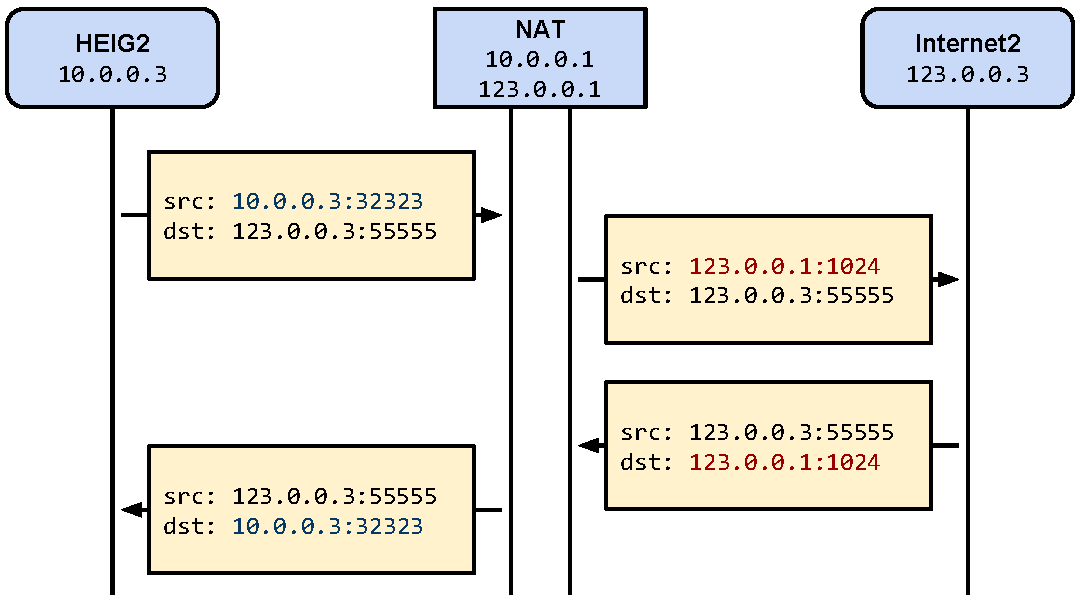
\includegraphics[width=15cm]{img_nat}
\end{center}

\section{Auto-évaluation}

Nous considérons avoir atteint les objectifs de ce laboratoire.

\end{document}